\documentclass[12pt,english]{article}
\usepackage[T1]{fontenc}
\usepackage[latin9]{inputenc}
\usepackage[toc,page]{appendix}
\usepackage{geometry}
\geometry{verbose,tmargin=1.5in,bmargin=1.5in,lmargin=1.5in,rmargin=1.5in}
\usepackage{bm}
\usepackage{amstext}
\usepackage{comment}
\usepackage{amsmath}
\usepackage{hyperref}
\hypersetup{
     colorlinks = true,
     citecolor = navy,
     linkcolor = navy,
     urlcolor=navy
}
\usepackage{adjustbox}
\usepackage[space]{grffile}
\usepackage{setspace}
\usepackage[normalem]{ulem}
\usepackage{nicematrix}
\usepackage{xcolor}
\usepackage{soul}
\usepackage{arydshln}
\usepackage{dsfont}
\usepackage{refstyle}
\usepackage[capitalize,nameinlink]{cleveref}
\usepackage{setspace}
\usepackage{bbm}
\usepackage[tableposition=t]{caption} % ensures caption of longtables is normalsized.
\usepackage{mathpazo} % add Palatino font
\usepackage{longtable}
\usepackage{amssymb}
\usepackage{amsfonts}
\usepackage{amsmath}
%\usepackage[margin=1in]{geometry} % to set margins
\usepackage{scalefnt}
\usepackage{wrapfig}
\usepackage{graphicx}
\usepackage{graphics}

%\usepackage{subfigure}
\usepackage{lscape}
\usepackage{pdflscape}
\usepackage{multirow}
\usepackage{array}
\usepackage{rotating}
\usepackage{bibunits}
\usepackage{fix-cm}
\usepackage{float}
\floatplacement{table}{H}
\usepackage{epsfig}
\usepackage{epstopdf}
\usepackage{refstyle}
\usepackage{tikz}
\usepackage{booktabs}
\usepackage{tabularx}
\usepackage{array}
\newcolumntype{x}[1]{>{\raggedleft\arraybackslash}p{#1}}%
\newcolumntype{d}[1]{>{\centering\arraybackslash}p{#1}}%
\newcolumntype{y}[1]{>{\raggedright\arraybackslash}p{#1}}%
\usepackage{verbatim}
%\epstopdfsetup{suffix=}
\setcounter{MaxMatrixCols}{10}
\usepackage[longnamesfirst,authoryear]{natbib}
\newenvironment{proof}[1][Proof]{\noindent \textbf{#1.}}{\rule{0.5em}{0.5em}}
\setlength{\topmargin}{-0.80in} \setlength{\textheight}{9.50in}
\setlength{\evensidemargin}{.0in} \setlength{\oddsidemargin}{.0in}
\setlength{\textwidth}{6.85in}
\setlength{\voffset}{0.4cm}
\setlength{\hoffset}{-0.5cm}
\usepackage{setspace}
\usepackage{afterpage}
\usepackage[flushleft]{threeparttable}
\usepackage{tabulary}
%\usepackage[titletoc,title]{appendix}
\usepackage[bottom]{footmisc}
\usepackage{color}
	\definecolor{maroon}{RGB}{128,0,0}
	\definecolor{navy}{RGB}{0,0,165}
	\definecolor{lb}{RGB}{150,165,190}
	\definecolor{bluenice}{rgb}{0.25,0.51,0.76}
	\definecolor{rednice}{rgb}{0.85,0.26,0}
	\definecolor{orangenice}{HTML}{EB811B}
	\definecolor{greennice}{HTML}{14B03D}
\usepackage{colortbl}
\usepackage{caption}
\usepackage{subcaption}
\usepackage{placeins}
\usepackage{nicefrac}
%\usepackage{chngcntr}
\newtheorem{assumption}{Assumption}
\newtheorem{definition}{Definition}
\usetikzlibrary{matrix,decorations.pathreplacing,arrows.meta,positioning}

\newcommand{\vy}{\underline{y}}
\newcommand{\ve}{\underline{\epsilon}}
\newcommand{\A}[1]{\mathbold{A_{#1}}}
\newcommand{\D}[1]{\mathbold{D_{#1}}}
\newcommand{\C}[1]{\mathbold{C_{#1}}}
\newcommand{\B}[1]{\mathbold{B_{#1}}}
\newcommand{\R}[1]{\mathbold{R_{#1}}}

%\newtheorem{definition}{Definition}
\begin{document}
\title{Two sector examples of calculating CPI}
\author{N}
\maketitle

\paragraph{Purpose:} Provide a 2 sector example where we see what the current CPI aggregation method does. I will show that it doesn't work as it should but that switching to weighting up value-added inflation with value-added weights will work without issue. I then outline how to code this up.

\section{Horizontal Economy -- Shapiro works well}

Let's imagine the case as set out in the diagram below.

\begin{tikzpicture}[>=stealth, node distance=2.5cm]
\tikzset{
  box/.style={
    draw,
    rectangle,
    minimum width=5.2cm,
    minimum height=5.2cm,
    align=center
  }
}

% Nodes
\node[draw, rectangle, text width=4cm, align=center] (s1) {Sector 1\\ (positive supply\\ = $2x$\%)};
\node[draw, rectangle, below of=s1,text width = 4cm,align=center] (s2) {Sector 2\\ (positive demand\\ = $4x$\%)};
\node[draw, rectangle, right=4cm of s1] (c) {Consumer};

% Arrows
\draw[->] (s1) -- node[midway, above] {$\tfrac{1}{2}$} (c.west);
\draw[->] (s2.east) -- node[midway, below] {$\tfrac{1}{2}$} (c.west);

\end{tikzpicture}

Here we have two sectors \emph{horizontally} selling a good to the household. 

Let's imagine that sector 1 has a positive supply shock and sector 2 has a negative demand shock. Let's imagine that the supply shock \emph{lowers} sector 1 prices by $2x$\% and the sector 2 demand shock \emph{raises} sector 2 prices by $4x$\%.

We can calculate CPI as:

\[
	\pi^{CPI} = -\frac{1}{2}2x + \frac{1}{2}4x = x
\]

With these numbers, we would have demand contributing $+4x$ to CPI and supply $-2x$ to CPI.

How do we calculate this formally? Well we create a vector (matrix when there are multiple time periods) indicating if the sector has experienced mostly a demand shock or supply shock. Call this $\underline{D}$ and let $D_i=1$ when it has experienced mostly a demand shock. Then we take the expenditure weights $\omega_{PCE}\equiv \begin{bmatrix} \frac{1}{2} & \frac{1}{2}\end{bmatrix}'$ and the sectoral CPI changes:

\begin{align*}
	\pi_{Demand} &=\sum_i D_i \omega_{PCE,i} \pi_i = 0\times \frac{1}{2}\times \left(-2x\right)+ 1 \times \frac{1}{2}\times 4x = 2x\checkmark\\
	\pi_{Supply} &=\sum_i (1-D_i) \omega_{PCE,i} \pi_i = 1\times \frac{1}{2}\times \left(-2x\right)+ 0 \times \frac{1}{2}\times 4x = -x\checkmark\\	
\end{align*}
where we can see that $\pi_{Demand} + \pi_{Supply} = \pi_{CPI}$. 

Note that ShapirIO is the same because there is no IO to correct for. Let's now see if we get it for the vertical economy.

\section{Vertical Economy -- does ShapirIO work well}

Let's switch to a vertical economy like the following diagram:

\begin{tikzpicture}[>=stealth, node distance=5cm]
\tikzset{
  box/.style={
    draw,
    rectangle,
    minimum width=5.2cm,
    minimum height=5.2cm,
    align=center
  }
}
% Nodes
\node[draw, rectangle, text width=4cm, align=center] (s1) {Sector 1\\ (positive supply\\ = $2x$\%)};
\node[draw, rectangle, right of=s1, text width=4cm, align=center] (s2) {Sector 2\\ (Net positive demand = $x$\%)};
\node[draw, rectangle,below =2cm of s2, text width=4cm, align=center] (sVA) {Value Added\\ (positive demand\\ = $4x$\%)};
\node[draw, rectangle, right of=s2, text width=4cm, align=center] (c) {Consumer};

% Arrows
\draw[->] (s1) -- node[midway, below] {$\tfrac{1}{2}$}  (s2);
\draw[->] (sVA) -- node[midway, right] {$\tfrac{1}{2}$}  (s2);
\draw[->] (s2) -- (c);

\end{tikzpicture}

In this vertical economy, note that sector 2's output price is identical to CPI. If we were doing Shapiro we would be getting:

\begin{align*}
	\pi_{Demand} &= 0 \times 0 \times -2x + 1 \times 1 \times x = x\\
	\pi_{Supply} &= 1 \times 0 \times -2x + 0 \times 1 \times x = 0\\	
\end{align*}
which is incorrect for the exact reasons we wanted to adjust Shapiro -- it misses IO interconnections.

OK, so let's do our IO corrections. There are two approaches: Adjust $D$ and switch to value added prices.

\paragraph{Adjust D:} This approach does the same aggregation as Shapiro but uses a $D$ that reflects the breakdown between supply and demand shocks along the IO network. \emph{Crucially, it does not distinguish between sectors with price rises or falls.}

So in this case, we would correct sector $2$ based on the fact that its own demand shock is only half of its output price. This would give us:

\[
	\tilde{D} = \begin{bmatrix}
		0\\
		\frac{1}{2}
	\end{bmatrix}
\]
Then if we use this $\tilde{D}$ matrix to calculate supply and demand inflation we would get:

\begin{align*}
	\pi_{Demand} &= 0 \times 0 \times -2x + \frac{1}{2} \times 1 \times x = \frac{x}{2}\neq 4x\\
	\pi_{Supply} &= 1 \times 0 \times -2x + \frac{1}{2} \times 1 \times x = \frac{x}{2}\neq -x\\	
\end{align*}

The reason this is incorrect is that we used the wrong $\tilde{D}$. To see this, let $\tilde{D} = \begin{bmatrix}
		0&
		2
	\end{bmatrix}'$. Now we have:

\begin{align*}
	\pi_{Demand} &= 0 \times 0 \times -2x + 2 \times 1 \times x = 2x\checkmark\\
	\pi_{Supply} &= 1 \times 0 \times -2x + (1-2) \times 1 \times x = -x \checkmark\\	
\end{align*}

So one option to fix this is to allow for negative $\tilde{D}$ when the upstream sector has a price fall. But I think there is an easier way:

\paragraph{Switch to Value Added Prices/Inflation:} Next, let's revert to a indicator vector for demand shocks $\underline{D}$ but instead of using $\omega_{PCE}$ and $\pi_i$ (output price inflation in each sector), we will use the value added weights for CPI which are:
\[
	\omega_{VA,i} = \begin{bmatrix}
		\frac{1}{2}\\\frac{1}{2}
	\end{bmatrix}
\]

And the inflation we will use will be value added inflation calculated as:

\[
	\pi_{VA} = \begin{bmatrix}
		-2x\\4x
	\end{bmatrix}
\]

Now the calculation is given by:

\begin{align*}
	\pi_{Demand} &= 0 \times \frac{1}{2} \times -2x + 1 \times \frac{1}{2} \times 4x = 2x\checkmark\\
	\pi_{Supply} &= 1 \times \frac{1}{2} \times -2x + 0 \times \frac{1}{2} \times 4x = -x \checkmark\\	
\end{align*}

And we are good! 

Note that this approach is much simpler than the previous one so let me outline a set of coding steps to operationalize this.

\section{Implementing the new calculations}

Let's start at the code where we have $\mathbold{D}\in \{0,1\}$ -- our classification of shocks as either mostly demand or supply (and not in-between), $\omega_{VA,i,t}$ and $\{P_{VA,i,t}\}_{i,t}$ -- our time series data of value added \emph{prices}. But before we begin, let's note that there is a small problem:

\begin{enumerate}
	\item CPI inflation in Shapiro is calculated linearly: $\pi_{CPI,t} = \sum_i \omega_{PCE,i,t-1} \times \pi_{i,t}$. I used a difference formula in the note before but let's stick with this one. [Tony, do we use official CPI data at any point in the analysis? If so, does either this formula or the one I gave you earlier match it exactly?]
	\item But our relationship between output prices $P_{i,t}$ and value added prices $P_{VA,i,t}$ is \emph{logarithmic}!
	\[
		\log(\underline{P}_t) = \mathbold{\Theta} \log(\underline{P}_{VA,t})
	\]
\end{enumerate}

The correct formula for output price inflation in each sector $i$ is given by:

\begin{align*}
	\pi_{i,t} &\equiv \frac{P_{i,t}}{P_{i,t-1}}-1 = \frac{\prod_j P_{VA,j,t}^{\theta_{i,j}}}{\prod_k P_{VA,j,t-1}^{\theta_{i,k}}}-1\\
	&=\prod_j \left(\frac{P_{VA,j,t}}{P_{VA,j,t-1}}\right)^{\theta_{i,j}}-1\\
	&=\prod_j \left(\frac{P_{VA,j,t}}{P_{VA,j,t-1}}-1\right)^{\theta_{i,j}} & \text{because }\sum_j \theta_{i,j}=1\text{.  [but please confirm!]}\\
	&=\prod_j \pi_{VA,j,t}^{\theta_{i,j}}
\end{align*}

CPI in terms of $\pi_{VA,j,t}$ is therefore:

\begin{align*}
	\pi_{CPI,t} = \sum_i \omega_{PCE,i}  \prod_j \pi_{VA,j,t}^{\theta_{i,j}}
\end{align*}

This is no-longer linear in $\pi_{VA,j,t}$!!!

There are two options: 

\begin{enumerate}
\item approximate the equation as:
\begin{align*}
	\pi_{CPI,t} &\approx \sum_i \omega_{PCE,i}  \sum_j\theta_{i,j} \pi_{VA,j,t}\\
	&= \sum_j \underbrace{\left(\sum_i \omega_{PCE,i} \theta_{i,j}\right)}_{\equiv \omega_{\pi_{VA,j,t}}}\pi_{VA,j,t}
\end{align*}


\item Continue with the non-linear version to get an exact match
\end{enumerate}

I recommend we start with the approximation, check it is accurate and if not, do both.

\subsection{Steps for the approximated method}

\begin{enumerate}
	\item Verify that $\log(\underline{P}_t) = \mathbold{\Theta} \log(\underline{P}_{VA,t})$, $\sum_i \omega_{PCE,i}=1$ and that $\sum_j \theta_{i,j}=1$ for all $i$ (simpler to just check $\mathbold{\Theta}\underline{1} = \underline{1}$ where $\underline{1}$ is a vector of ones.
	\item Calculate $\underline{P}_{t}^{approx} \equiv \mathbold{\Theta} \underline{P}_{VA}$ (note that we are ignoring the logs here).
	\item Check the differences between $\underline{P}_t$ and $\underline{P}_{t}^{approx}$. Specifically let's calculate the mean absolute difference and largest absolute difference. {\bf If these are very large, we should be worried but still continue to the next step. If they are larger than 100\% or -100\% we are probably going to be in trouble....} 
	\item Calculate the (approximated) CPI weights on value-added inflation (matrix method probably quicker): 
	\[
		\omega_{VA,i,t}\approx \sum_j \omega_{PCE,j,t-1} \theta_{j,i} = \underline{\omega}_{PCE,t-1}'\mathbold{\Theta}
	\]
	\item Check these weights sum to 1 (see proof just after this for why they should):
	\begin{align*}
		\sum_i\omega_{VA,i,t} = \sum_i\sum_j \omega_{PCE,j,t-1} \theta_{j,i} = \sum_j \omega_{PCE,j,t-1} \underbrace{\sum_i \theta_{j,i}}_{=1} = \sum_j \omega_{PCE,j,t-1}=1
	\end{align*}
	{\bf If these don't sum to 1 properly email Nick}	
	\item Calculate VA inflation and output price inflation (BEA price data) as:
	\[
		\pi_{VA,i,t} = \frac{P_{VA,i,t}}{P_{VA,i,t-1}}	
	\]
	and 
	\[
		\pi_{i,t} = \frac{P_{i,t}}{P_{i,t-1}}	
	\]	
	\item Calculate approximate CPI inflation and compare to Shaprio's CPI inflation calculation:
	\begin{align*}
		\pi_{CPI,t} &=  \sum_i \omega_{PCE,i,t-1} \pi_{i,t}\\
		\pi_{CPI,t}^{approx} &= \sum_i \omega_{\pi_VA,i,t-1}\pi_{VA,i,t}
	\end{align*}
		
	\item Check the differences between $\pi_{CPI,t}$ and $\pi_{CPI,t}^{approx}$. Specifically let's calculate the mean absolute difference and largest absolute difference. {\bf We want an average error less than 3\% and a max error less than 10\%. }
	If these are satisfied, we can skip the exact method.
	\item Now we need demand driven and supply driven inflation. These are calculated as:
	
	\begin{align*}
		\pi_{Demand} &= \sum_i D_i \omega_{\pi_{VA},i,t-1} \pi_{VA,i,t}\\
		\pi_{Supply} &= \sum_i (1-D_i) \omega_{\pi_{VA},i,t-1} \pi_{VA,i,t}\\
	\end{align*}
\end{enumerate}

\subsection{Steps for the exact method}
\begin{enumerate}
	\item {[If not already done]} Verify that $\log(\underline{P}_t) = \mathbold{\Theta} \log(\underline{P}_{VA,t})$, $\sum_i \omega_{PCE,i}=1$ and that $\sum_j \theta_{i,j}=1$ for all $i$ (simpler to just check $\mathbold{\Theta}\underline{1} = \underline{1}$ where $\underline{1}$ is a vector of ones.
	\item Calculate VA inflation and output price inflation (BEA price data) as:
	\[
		\pi_{VA,i,t} = \frac{P_{VA,i,t}}{P_{VA,i,t-1}}	
	\]
		and 
	\[
		\pi_{i,t} = \frac{P_{i,t}}{P_{i,t-1}}	
	\]	
	\item Calculate CPI inflation via the Shapiro method for comparison purposes later.
	\[
		\pi_{CPI,t} =  \sum_i \omega_{PCE,i,t-1} \pi_{i,t}
	\]
	\item Calculate the following concepts:
	\begin{align*}
		\pi_{i,t}^{IO} &= \prod_j \pi_{VA,j,t}^{\theta_{i,j}} & \text{Should equal }\pi_{i,t}\text{ (output inflation for sector }i\text{)}\\
		\pi_{i,Demand,t}^{IO} &= \sum_j \pi_{VA,j,t}^{D_{j,t}\theta_{i,j}}\\
		\pi_{i,Supply,t}^{IO} &= \sum_j \pi_{VA,j,t}^{(1-D_{j,t})\theta_{i,j}}\\
		\pi_{i,Interactions,t}^{IO} &= \pi_{i,t}^{IO} - \pi_{i,Demand,t}^{IO} - \pi_{i,Supply,t}^{IO}
	\end{align*}	
	The first should be the exact calculation of output price inflation. The second and third are the contributions of demand and supply shocks to output prices in sector $i$. The fourth is to account for the fact that supply and demand's contribution to inflation in each sector is **not** linarly separable. That means that $\pi_{i,t} \neq \pi_{i,Demand,t}^{IO} + \pi_{i,Supply,t}^{IO}$ 
	{\bf Note: these are not linearly separable! I will elaborate later.}
	\item Check the following:
	\begin{itemize}
		\item Sectoral inflation calculated via $\pi_{VA,j,t}$ is equal to output price inflation from BEA $\pi_{i,t}^{IO} = \pi_{i,t}$.
		\item Overall output inflation in each sector equals \emph{the product} of demand and supply driven inflation: $\pi_{i,t}^{IO} = \pi_{i,Demand,t}^{IO}\cdot \pi_{i,Supply,t}^{IO}$
	\end{itemize}
	Email Nick if they are not equal
	\item Now we can calculate the contribution of demand and supply shocks to inflation:
	\begin{align*}
		\pi_{CPI,t} &= \sum_i \omega_{PCE,i,t-1} \pi_{i,t}^{IO}\\
		\pi_{CPI,Demand,t} &= \sum_i \omega_{PCE,i,t-1} \pi_{i,Demand,t}^{IO}\\
		\pi_{CPI,Supply,t} &=\sum_i \omega_{PCE,i,t-1} \pi_{i,Supply,t}^{IO}\\
		\pi_{CPI,Interactions,t} &=\sum_i \omega_{PCE,i,t-1} \pi_{i,Interactions,t}^{IO}\\
	\end{align*}
	\item Confirm that these three contributions all add up to CPI
	\[
		\pi_{CPI,t} = \pi_{CPI,Demand,t} + \pi_{CPI,Supply,t} + \pi_{CPI,Interactions,t} 
	\]
	\item plot them and let's see what we get! Hopefully interactions are not super large....
\end{enumerate}

\section{Earlier Incorrect Version}

\begin{enumerate}
	\item Verify that $\sum_i \omega_{VA,i,t} P_{VA,i,t} = P_{CPI,t}$ (or that $\sum_i \omega_{i,PCE} P_{i,t} = \sum_i \omega_{VA,i,t} P_{VA,i,t}$)
	\item Calculate value added \emph{inflation}: 
	\[
		\pi_{VA,i,t} = \frac{P_{VA,i,t}}{P_{VA,i,t-1}}-1
	\]
	\item Calculate some inflation-based expenditure weights:
	\[
		\omega_{\pi_{VA},i,t} = \frac{\omega_{VA,i,t}P_{VA,i,t-1}}{\sum_j \omega_{VA,j,t-1}P_{VA,j,t-1}}
	\]
	
	based on the following logic:
	
	\begin{align*}
		\pi_{CPI,t} &=\frac{P_{CPI,t}}{P_{CPI,t-1}} = \frac{\sum_i \omega_{VA,i,t} \textcolor{blue}{P_{VA, i,t}}\textcolor{red}{\frac{P_{VA, i,t-1}}{P_{VA, i,t-1}}}}{\sum_j \omega_{VA,j,t-1} P_{VA, j,t-1}} = \sum_i \left(\frac{\omega_{VA,i,t}\textcolor{red}{P_{VA,i,t-1}}}{\sum_j \omega_{VA,j,t-1} P_{VA, j,t-1}} \times \textcolor{blue}{\pi_{VA,i,t}}\right)
	\end{align*}	
	
	\item Verify these weights sum to 1: $\sum_i \omega_{\pi_{VA},i,t}=1$.
	\item Verify that with these weights and value added inflation we recover CPI inflation $\pi_{CPI} = \sum_i \omega_{\pi_{VA},i,t} \pi_{VA,i,t}$ (another check is whether $\sum_i \omega_{\pi_{VA},i,t} \pi_{VA,i,t} = \sum_i \omega_{\pi_{PCE},i,t} \pi_{i,t}$.)
	\item Then use these weights with the original $D$ to calculate demand and supply:
	
	\begin{align*}
		\pi_{Demand} &= \sum_i D_i \omega_{\pi_{VA},i,t} \pi_{VA,i,t}\\
		\pi_{Supply} &= \sum_i (1-D_i) \omega_{\pi_{VA},i,t} \pi_{VA,i,t}\\
	\end{align*}
\end{enumerate}

\end{document}